\documentclass[11pt,letterpaper,english]{article}

\usepackage[margin=1.0in]{geometry}
\usepackage{helvetica}
\usepackage[table]{xcolor}
\usepackage{graphicx}

\title{Effects of Economic Relase Data on Market Health Indicators}
\author{Ian Clark}
\date{}

\begin{document}
\maketitle

\section{The ISM Manufacturing Index}
With a consensus range from 53.5 to 56.5 and a mean consensus of 55, the data for the ISM Manufacturing Index was released lower than predicted at 53.5. However, from this number we can assume that we are still in economic expansion (as of a month ago). These numbers, although having fallen, still prove promising, for the fact alone that we remain in an economic expansion. When coupled with the employment data later, we can assume to be growing at a steady pace.

\subsection{Effects Upon the Market}
Affects upon the S\&P 500 were questionable at best, as the market climate (for the day) was already slipping into a turmoil of sorts because of news concerning the European Central Bank and decisions from Greece's new Finance Minister Yanis Varoufakis. Regardless, operating under the (naïve) assumption that a negative/positive change in the ISM Manufacturing Index would negatively/positively affect the S\&P 500, we can see correlation--$\Delta{ISM} = -1.6$ and $\Delta{S\&P} = -15.77$ or $\%\Delta{S\&P} = -0.79$. Admittedly, these numbers are opening and low amounts and the S\&P index ended the day on a net gain in value.

\vspace{5mm}

\noindent One may assume that when the ISM releases promising numbers, fewer investors will opt into purchasing risk-free bonds, or the 10 year treasury bond. Since the ISM fell, the opposite should theoretically be the result. As stated earlier, because of the climate within the markets, one should expect additional variance in the 10 year treasury price because of Europe. With an opening price of 1.67, the 10 year treasury spread widely throughout the day: from 1.65 at the lower-bound and 1.71 at the upper-bound, the 10 year ended up spreading an entire 6 basis points. The price of the bond on the 2\textsuperscript{nd} was far too variable to assert the ISM was the sole contributing factor.

\section{The Employment Situation}
The employment situation data has all-around been fantastic, with consistently high revisions ranging from November's astounding revisions in non-farm month-to-month payroll to February's release data. Considering the trend (please see below data), further positive revisions seem both feasible and plausible.

\begin{center}
    \begin{tabular}{| c | c | c | c |}
    \hline
    Month       & Original (1000s) & Revised (1000s) & Difference (1000s) \\ \hline
    November    & 353 & 423 & \cellcolor{green}{+70} \\ \hline
    December    & 252 & 329 & \cellcolor{green}{+77} \\ \hline
    January     & 321 & 353 & \cellcolor{green}{+32} \\ \hline
    February    & 257 & \cellcolor{black}{} & \cellcolor{black}{} \\ \hline
    \end{tabular}
\end{center}

\noindent Moreover, the Unemployment Level (the u3) has risen (employment has increased) from $5.6\%$ to $5.7\%$, albeit this seems to indicate the economy is in such a promising position that many previously discouraged workers have opted to return to the job search, thus creating a slight convergence between the u3 and u6 employment rates. 
Contributing to this, we saw a rise from $62.7\%$ labor force participation to $62.9\%$. This statistic, however, is not as impressive, as the trend has been for labor force participation to remain near $62.9\%$, as seen below:

\vspace{10mm}
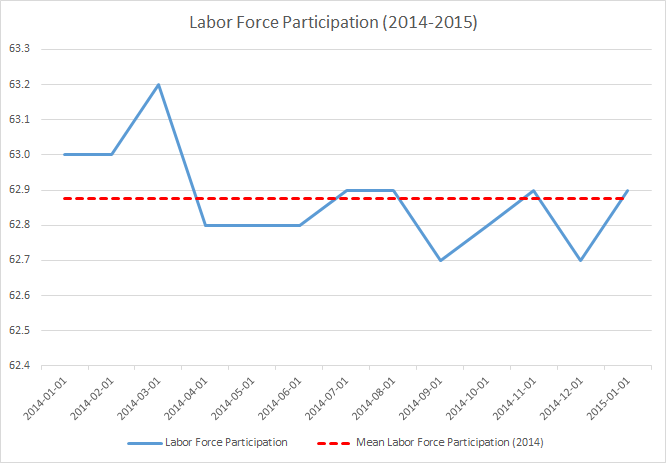
\includegraphics[scale=0.85]{LaborForceParticipation.png}
\vspace{10mm}

\noindent As well, the other promising statistic within the data is the month-to-month Average Hourly Earnings, which rose a total of $.5\%$--exceeding the consensus range ($.1\%$ to $.5\%$) by an entire $20\%$. From September to December of 2014, the United States experienced positive net gains across all workers\footnote[1]{The Employment Cost Index, http://www.bls.gov/web/eci/ecconstnaics.txt}, so for the foreseeable future, this trend may well continue.

\subsection{Effects Upon the Market}
Given the positive nature of the Employment Situation data, one could reasonably assume positive gains within the S\&P 500, as these numbers can sensibly predict growth within the economy. As such, one could operate under the (naïve) assumption that when the news is positive, so is the reaction upon the market. The high of February 6\textsuperscript{th} for the S\&P 500 was 2072.4, yet the market opened at 2062.28--yielding a $\Delta{S\&P}$ of $0.49\%$. While the employment numbers may have had a positive effect on the S\&P 500 for a duration, the duration was not long-lasting as the S\&P 500 closed at 2055.47--a loss for the day of $0.33\%$.

\vspace{5mm}

\noindent While the ISM's effects may have gone unnoticed on Monday, the Payroll data seemed to have highly affected the 10 year treasury prices. Climbing an entire 12 basis points, the 10 year opened at 1.82 and closed at 1.94. Because the Federal Reserve has recently been hinting at future increases to key interest rates, this strong report caused expectations of the Fed increasing interest rates sooner rather than later, thus increasing bond prices.

\section{Conclusion and Personal Thoughts}
I feel that the market's reaction to other news on February 2\textsuperscript{nd} is far too unreliable to assert that the ISM had such a pronounced effect. I do, however, feel that in years to come the ISM can prove to be a very useful metric for gauging economic health and appreciate the "boots to the ground," approach of polling purchasing managers. On the other hand, having lag inherently placed into the model can make it slightly less reliable--although still an overall decent indicator of economic health.
\vspace{5mm}

\noindent On behalf of the payroll statistics, some of the best news came from past revisions, as detailed by the graph. With November being revised to a total of 423,000, we have had some of the strongest growth in non-farm payrolls over the past four months since 1997\footnote[1]{1,230,000 since November versus 1,462,000 in 1997 September through December}. I'm personally excited about the numbers in the payroll statistics--at least more so than the disappointing ISM--mostly for the labor force participation rate and the Average Hourly Earnings. As shown in the Bureau of Labor Statistics Report\footnote[2]{http://www.bls.gov/web/eci/ecconstnaics.txt}, we could see a period of loss and stagnation within earlier months of 2014 in median wage growth, but we can now see a period of consistent wage growth amongst all workers.
\vspace{2.5mm}

\noindent Given the news in Greece, I feel there were strange happenings--which probably wouldn't have happened otherwise--concerning the 10 year treasury and the S\&P 500 because the S\&P 500 feel at the end of the 6\textsuperscript{th}, whereas they rose on the 2\textsuperscript{nd}. I follow the belief that stocks wouldn't have fallen after such great news if a Greek disaster was not looming on the horizon.


\newpage
\begin{thebibliography}{9}
\bibitem{Bloomberg}
    Bloomberg,
    \emph{http://www.bloomberg.com/markets/economic-calendar/}.
\bibitem{BLS Worker Data}
    Bureau of Labor Statistics (Employment Cost),
    \emph{http://www.bls.gov/web/eci/ecconstnaics.txt}.
\bibitem{BLS Historic Data}
    Bureau of Labor Statistics (Historical Payroll),
    \emph{http://www.bls.gov/news.release/empsit.nr0.htm}.
\bibitem{Yahoo Finance}
    Yahoo Finance,
    \emph{http://finance.yahoo.com/}.
\end{thebibliography}

\end{document}